\documentclass{article}
\usepackage{amsmath}
\usepackage{hyperref}
\usepackage{tikz}
\usepackage{siunitx}
\usepackage{array}
\begin{document}

\title{EMI on Lower HF}
\author{David Rowe VK5DGR}

\maketitle

\section{Introduction}
 
Throughout the 20th century HF radio receiver technology evolved with the aim of detecting distant, narrow band signals.  Radio noise sets the limits of detection, and was assumed to be from natural sources or the receiver itself.  However in the early 21st century, noise from human activity now dominates the detection problem.  We are no longer seeking to maximise signal-to-noise ratio (SNR), but signal to EMI ratio (SER).

We are slowly losing the ability to use analog SSB in urban areas.  Many Hams report S9 noise levels, $9 \times 6 = 54$ dB higher than a quiet S0 country station.  Consequently, digital modes that can operate operate at low SNRs are becoming popular.

Our target radio signals are from distant sources, weak, narrow band, and evolve slowly in time. Human generated radio noise tends to be very strong, wideband, with a time domain envelope that evolves quickly in time.  It is often radiated from nearby sources, such as power lines lines and house wiring a few meters from our antenna.  Some EMI has significant structure, so can be interpreted as an interfering signal, rather than random noise.

There are a lot of on-line opinions, hearsay, rules of thumb, and subjective reports on this topic.  I have found this topic to be very complex, with many inter-related variables. Everyone else seems to work DX ok. I often wondered if my site was the exception - is it just my house or suburb?  

This report is a my personal study, written to further my understanding of the topic, and hopefully improve conditions at my home station. No claim of any original work is made.

\subsection{Summary}

\begin{enumerate}
\item S-meters can't be trusted \cite{vu2nsb_s_meter}, you'll need a calibrated way to measure noise power at your site.
\item Measure your ambient noise figure $F_a$ and compare to P.372 \cite{itu372-16}.
\item If your noise is AWGN and your $F_a$ is similar to P.372 it's probably city wide noise, rather than something local. Congratulations you are doing as well as can be reasonably expected. Your options are a directional antenna, or moving your antenna to the country.
\item If you see harmonics on your waterfall (and hear tones as your tune across the band) it's PWM and likely very local.
\item If it's rapid clicks or buzzing it's impulse noise which is also local, but can travel down power lines around suburbs. 
\item To address PWM and impulse local noise, position your antenna at least 6m from any buildings, power and phone lines.  Look for and address any common modem feedline issues, use a balun on your dipole, or use antennas with good balance (like loops).  Try Diversity.  Your noise blanker might work for impulse noise.  A small loop antenna might help as it is easier to place away from noise sources than a wire antenna.
\item If possible, find and remove the local noise sources.
\end{enumerate}

\begin{table}[h]
\centering
\begin{tabular}{ | m{1.2cm} | m{4cm} | m{3cm} | m{2cm} |}
 \hline\hline
 Name & Characteristics & Example & Sound \\
 \hline
 AWGN & Constant in time and frequency & Natural noise, or sum of many sources & Ssshhh \\
 \hline
 Impulse & Short pulses far apart in time $R<B$, wideband in frequency & Power lines, Ignition & clicks or buzzing \\
\hline PWM & Short pulses close together in time $R>B$, harmonics in frequency & Switch mode power supplies & tones or hash \\
 \hline
\end{tabular}
\caption{How I classify noise. AWGN is Additive White Gaussian Noise, PWM is Pulse Width Modulation, $R$ is the frequency of the noise pulses, $B$ is your receiver bandwidth.}
\label{table:noise_classes}
\end{table}

\subsection{Selected References}

References I recommend are ITUT-R P372 \cite{itu372-16}, the W8JI web site \cite{w8ji_radio_noise} for a concise overview of HF noise and small loop antenna myths; and the web site of LZ1AQ \cite{lz1aq} for his studies on small loop antenna arrays. After some experimentation \cite{rowetel_noise_city} I've settled on the approach suggested by Owen Duffy \cite{duffy_lig} and Basu \cite{vu2nsb_s_meter} - comparing my ambient noise floor to P.372 to check my baseline, then seeing what I can do about local noise sources. John Fallows VE6EY \cite{ve6ey} has some fine material on noise reductiuon using diversity receivers on his blog and YouTube channel.

\section{Radio Noise Signals from Human Activity}

Table \ref{table:human_noise} is a summary of human generated noise sources.  The values are approximate and based on my experience - your mileage may vary!  This categorisation gives us some insight that can be used to classify signals, consider their impact, and possible attacks.

The Time and Frequency columns describe the distribution of energy in time and frequency, for example power line arcing can cause clicks similar to atmospheric lightning.  The noise signal consists of short, powerful time domain pulses that are randomly distributed in time, resulting in wideband energy uniformly distributed in frequency. It may be identified and removed via noise blanking techniques.

In contrast DSL signals radiated from leaky phone lines looks like noise in the time domain and frequency domain, making it particularity hard to identify and remove.  It is very similar to AWGN from natural noise sources.

Bandwidth relates the rate $R$ of the noise pulses to the bandwidth $B$ of a typical SSB HF receiver (around 2000 Hz).  When $R<<B$, we tend to hear individual noise pulses, and separate pulses can be observed in a time domain plot of the receiver output waveform.  When $R>B$, we hear just a bandpass segment of the EMI signal, for example a tone from a PWM harmonic, or some modulated noise.

Our narrow band receiver smooths the time domain envelope of noise impulses. As $R$ relative to $B$ increase, our receiver smears the short time domain pulses (such as a PWM waveform) into a longer pulses with a smoother time domain envelope (such as damped sinusoids and in the limiting case AWGN noise), making the EMI signal harder to identify and remove.

For EMI signals to be detected by our receiver, we need a source of RF currents and a way of coupling those current into our antenna system (which includes the antenna and feed line).  On lower HF our antenna systems are typically located less than one wavelength from the source of RF currents so both near and far field coupling is possible, and indeed a combination of both seems likely.

If we position our receiver some distance from many noise signals, we get the sum of many signals added together, which converges to far field AWGN noise.  The level reduces with distance, so an effective attack is travelling to a country location, and operating a portable station for the day.

Domestic electricity lines appear to operate in a mode part way between transmission line and antenna.  RF does seem to propagate along them quite well, they then couple quite well into nearby antennas.  Likewise, DSL signals on ancient phone lines are poor transmission lines and reasonably effective antennas, radiating significant local EMI. A home with buried electricity lines and fibre or wireless supplying Internet is an effective attack on these sources.

\begin{table}[h]
\centering
\begin{tabular}{l l l l l l}
 \hline
 Name & Rate & Time & Frequency & Antenna & BW \\
 \hline
 Power Line & 1 Hz & random pulse & uniform & power lines & $R < B$ \\
 Downlights & 50-60 Hz & pulse train & harmonics & house wiring & $R < B$ \\
 SMPS & 10-300 kHz & pulse train & harmonics & house wiring & $R > B$ \\
 DSL & 1-12 MHz & AWGN & AWGN & phone lines & $R > B$ \\
 Urban Sum & lower HF & AWGN & AWGN & power lines & $R > B$ \\
 \hline
\end{tabular}
\caption{Summary of Radio signals from Human Activity}
\label{table:human_noise}
\end{table}

The modulation used in our desired target signals is a factor.  Digital modes can operate at lower SNRs than analog SSB.  Digital modes can also use Forward Error Correction (FEC), e.g. we can correct a bit error caused by a noise impulse wiping out one bit.  Digital modulation also has a threshold effect - once the interference is a few dB lower than the wanted signals, it's impact on bit errors is small. FM, FSK \& PSK are more robust to impulsive noise than amplitude modulated modes like SSB.  However digital modes (just like analog) can't penetrate high AWGN noise levels.

\section{EMI from Pulse Trains}
\label{pwm}

\subsection{Pulse Width Modulation}
\label{smps}

The PWM switch mode power supply is a ubiquitous source of interference.  Consider the Fourier Series of an ideal pulse train \cite{wikipedia_pulse}:
\begin{equation} \label{eq_pwm}
\begin{split}
x(t) &= Ad+\frac{2A}{\pi} \sum_{n=1}^{\infty} \frac{sin(\pi n d)}{n}cos(n \omega t) \\
     &= Ad+\frac{2A}{\pi} \sum_{n=1}^{\infty} \frac{x(t)}{n} cos(n \omega t)
\end{split}
\end{equation}
where $0<d<1$ is the duty cycle and $\omega=2 \pi R$ the fundamental frequency.  The Fourier series is a sequence of harmonics $cos(n \omega t)$, with the amplitude of each harmonic set by the $x(t)/n$ term. A typical value for $R$ is a few kHz to several hundred kHz. For example with R = 70kHz and $n=101$ we will have a harmonic at 7.1 MHz. The $1/n$ factor means the power of each harmonic falls off slowly with frequency, e.g. the $n=100$ harmonic will be just $10log_{10}(1/100)=-20$ dB down compared to the fundamental ($n=1$) power, and the $n=101$ harmonic almost the same power at $10log_{10}(1/101)=-20.043$ dB down.

If the duty cycle $d$ is constant, then each harmonic is an unmodulated sine wave of constant amplitude. In practice $d$ is time varying, as the duty cycle is continuously adjusted by the power supply.  This leads to modulation of each harmonic $x(t)$, spreading the power to frequencies either side of the harmonic centre $n \omega$.

Let $d$ have a constant and time varying component:
\begin{equation}
d=d_c+ad(t)
\end{equation}
where $d(t)$, $|d(t)| \le 1$ is a PWM modulation function and $a$ is the peak amplitude of the modulation (ie the peak jitter of the PWM signal). For the $n$-th harmonic:
\begin{equation} \label{eq:pwm_n}
\begin{split}
x_n(t) &= sin(\pi n d) \\
       &= sin(\pi n (d_c+ad(t)) \\
       &= sin(\pi n d_c + \pi n a d(t)) \\
       &= sin(\pi n d_c + h d(t))  \\
     h &= \pi n a
\end{split}
\end{equation}
It can be seen that $h$ is strong function of $a$, as small changes are multiplied by $n \pi$. For example for $n=100, a=0.01, h = \pi$.  Thus with just 1\% jitter of the PWM signal, a cycle of $d(t)$ would modulate over the entire $\pm \pi$ range of the $sin()$ function.

We would like to estimate the spectrum of $x(t)$. First we consider small $h << 1$:
\begin{equation} \label{eq:small_h}
\begin{split}
x_n(t) &= sin(\pi n d_c)cos(hd(t)) + cos(\pi n d_c)sin(hd(t)) \\
       &\approx sin(\pi n d_c)(1 - (hd(t))^2/2) + cos(\pi n d_c)hd(t) \\
       &\approx sin(\pi n d_c) + hcos(\pi n d_c)d(t)
\end{split}
\end{equation}
The LHS is a constant term related to the mean duty cycle of the PWM signal, the RHS is linear modulation term, i.e. a small linear modulation about a mean set point.  When multiplied by the $n$-th harmonic $cos(n \omega t)$ in (\ref{eq_pwm}):
\begin{equation}
\begin{split} \label{eq:small_h2}
x_n(t)cos(n \omega t) &= \left[ sin(\pi n d_c) + hcos(\pi n d_c)d(t) \right] cos(n \omega t) \\
                      &= sin(\pi n d_c)cos(n \omega t)) + hcos(\pi n d_c)d(t)cos(n \omega t) \\
                      &= c_1 cos(n \omega t)) + c_2 d(t)cos(n \omega t) \\
                   c_1 &= sin(\pi n d_c) \\
                   c_2 &= hcos(\pi n d_c)
\end{split}
\end{equation}
By examining the different frequency terms we can estimate the spectrum of the PWM signal near the n-th harmonic. Note $c_1$ and $c_2$ are constants that do not affect the number of different frequency terms. The LHS of (\ref{eq:small_h2}) is a constant carrier term at the harmonic centre. The product of $d(t)cos(n \omega t))$ will produce images of the spectra of d(t) either side of $n \omega$. Thus (\ref{eq:small_h2}) is Amplitude Modulated (AM) signal.  For example if $d(t)$ is a random variable with maximum frequency $\omega_m$ radians, we would see a uniform noise spectrum over the interval $n \omega \pm \omega_m$, with a central "carrier" spectral line at $n \omega$. If $\omega_m > \omega/2$, the entire region between each harmonic will have additive white noise generated from the PWM signal.

For larger $h$, Equation \ref{eq:pwm_n} can be interpreted as Phase Modulation (PM) \cite{wikipedia_phase} of a zero frequency carrier. Assuming a random $d(t)$, the resulting spectra of $x(t)$ can be approximated using Carsons Rule, as having 98\% of it's power contained within $B_c=2(h+1)f_m$ Hz, where $f_m$ is the maximum frequency component of $d(t)$. When multiplied by the $cos(n \omega t)$ term, the PM signal will spread the power of the carrier over range of adjacent frequencies, replacing the PWM carrier in the small $h$ case with a wideband signal.

For example, let $a=0.02$ (a few percent jitter of the PWM duty cycle) and the bandwidth of the PWM control loop be $f_m=3$ kHz. At $n=100$ we have $h=\pi n a = 2\pi$, which implies a random deviation of $\pm 2\pi$ (two cycles of $sin()$), and an $x(t)$ bandwidth of $B_c=2(2 \pi+1)f_m = (4\pi+2)f_m = 43$ kHz.

\subsection{Discussion}

\begin{enumerate}
\item Given $h$ increases with $n$, we can expect to see AM type modulation either side of central harmonics lines at lower frequencies.  At intermediate frequencies a raised noise floor will be observed between harmonics.  As the frequency increases further the power of the harmonics lines will reduce and gradually be replaced by broadband noise.
\item With the common scenario of a receiver of bandwidth $B<R$, we would encounter sine wave "carriers" every R kHz as we tune.  Tuning between carriers would expect to hear a bandpass version of $d(t)$, this may or may not be white.  If not white, it may have structure we can exploit.
\item With a large number of PWM sources, the central limit theorem suggests the sum will converge to AWGN noise with very little structure in time or frequency.  This may the case with signals radiated from electricity power lines that are coupled to thousands of switch mode power supplies in a city.
\item In the local case, it is possible that switch mode PWM or impulse noise may dominate a particular receiving station.
\end{enumerate}

\subsection{Periodic Impulse Noise}

Section \ref{smps} explored the spectra of PWM power supplies which typically have a pulse rate $R$ greater than the receiver bandwidth $B$ (e.g. $B=2000$Hz for SSB signals on HF radio). A low frequency pulse train (such as ignition or $R=50 \ldots 60$ Hz impulses from domestic lighting) can also be interpreted as a pulse train with small duty cycle $d$, and $R<<B$.  In this case there will be a number of harmonics inside our receiver passband.  Consider (\ref{eq_pwm}), band pass filtered such that only harmonics $n_1 \ldots n_2$ remain:
\begin{equation}
\begin{split}
x(t) &= Ad+Ad\sum_{n=1}^{\infty} sinc(\pi n d) cos(n \omega t) \\
BPF \left[ x(t) \right] &= Ad\sum_{n=n_1}^{n=n_2} sinc(\pi n d) cos(n \omega t)
\end{split}
\end{equation}
Shifting down to baseband, and making the substitution $k=n-n_1$:
\begin{equation}
\begin{split}
BPF \left[ x(t) \right] cos(n_1 \omega t) &= \frac{Ad}{2} \sum_{k=0}^{n=n_2-n_1} sinc(\pi (k+n_1) d) cos(k \omega t) \\
&+ \frac{Ad}{2} \sum_{k=0}^{n=n_2-n_1} sinc(\pi (k+n_1) d) cos((k+n_1) \omega t) \\
&= b(t) + c(t)
\end{split}
\end{equation}
By applying a low pass filter we are left with the baseband term $b(t)$:
\begin{equation}
\begin{split}
b(t) &= \frac{Ad}{2} \sum_{k=0}^{n=n_2-n_1} sinc(\pi (k+n_1) d) cos(k \omega t) \\
     &= \frac{Ad}{2} + \frac{Ad}{2} \sum_{k=1}^{n=n_2-n_1} sinc(\pi n_1 d + \pi k d) cos(k \omega t)
\end{split}
\end{equation}
This expression is similar to the Fourier Series for a pulse train (\ref{eq_pwm}), but limited to $n_2-n_1$ harmonics by the bandwidth $B$ of the receiver.  The baseband signal $b(t)$ can therefore be interpreted as a periodic signal with the same period $\omega$ as the wideband periodic impulse noise $x(t)$.  The shape of the pulse train will be a modified version of the $x(t)$, as we are using a band pass set of $sinc()$ coefficients.  Given the duty cycle $d$ is likely to be small (e.g a $10 \mu$s pulse every 20ms), and $n_2-n_1 << n_1$, the coefficients are likely to be similar in amplitude across $n_1 \ldots n_2$, producing a high peak to average power (low duty cycle) ratio pulse train.

Given $d$ is small, and there is still significant power at high harmonic numbers, $A$ must be very large for these impulse noise sources.

\subsection{Attacks}

\begin{enumerate}
\item Estimation and subtraction of the signals. Key take away is mirror of $d(t)$ about harmonic centre. Estimation of signal from one sideband to cancel other, or from AM demodulation (envelope). This will be problematic when it's spread so far that we get energy from $n+1$, $n-1$ near harmonic $n$.  However in that case it may not be as annoying/strong.

\item Estimation of signal from adjacent harmonics.  Can we find $x_n(t)$ from $x_{n-1}(t)$?  $\omega$ and $n$ can be estimated from the spectrum.  A direct form solution is unlikely however the equations are differentiable so an iterative solution could be found.

\item Dual channel coherent removal (diversity receiver).

\item Noise blanking in the time domain.  This may be challenging with $R>100$ kHz, as the period becomes $< 10\mu$s, implying the need for a wide bandwidth and sample rate $>>100$ kHz in order to resolve individual noise pulses in the time domain.

\item Training of time domain pulses, correlation and removal.
\end{enumerate}

\section{Noise Blanker}

Consider a signal $x(t)$ consisting of a wanted sinusoidal signal and an unwanted impulse train that repeats every $1/R$ seconds.
\begin{equation}
x(t) = a_1 e^{j \omega_1 t} + a_{imp}\sum_{n=-\infty}^{\infty}\delta(t-n/R)
\end{equation}
To remove the impulse, a blanking pulse train $b(t)$ is applied.  Each pulse is $T$ seconds wide:
\begin{equation}
\begin{split}
b(t) &= 1 - p(t) \\
p(t) &= \sum_{n=-\infty}^{\infty}rect(t-n/R) \\
rect(t) &= 
	\begin{cases}
      1, & |t| <= T/2 \\
      0, & otherwise \\
	\end{cases} \\
\end{split}
\end{equation} 
The blanking pulse train removes the impulse pulse train such that:
\begin{equation}
\sum_{n=-\infty}^{\infty}\delta(t-n/R) b(t) = 0
\end{equation}
\begin{figure}[h]
\caption{Blanking Pulse $b(t)$ }
\vspace{5mm}
\label{fig:rect_time}
\centering
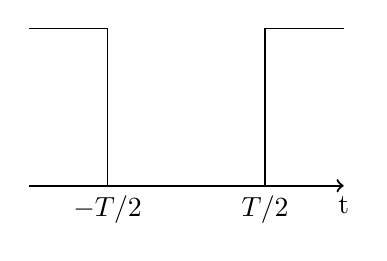
\begin{tikzpicture}
\draw[thick,->] (1,0) -- (5,0) node [below]{t};
\draw (1,2) -- (2,2) -- (2,0) node [below]{$-T/2$} -- (4,0) node [below]{$T/2$} -- (4,2) -- (5,2);
\end{tikzpicture}
\end{figure}

The pulse train $p(t)$ can be expressed as Fourier Series (\ref{eq_pwm})
\begin{equation}
\begin{split}
p(t) &= d+\frac{2}{\pi} \sum_{n=1}^{\infty} \frac{sin(\pi n d)}{n}cos(n \alpha t) \\
     &= d + d \sum_{n=1}^{\infty} sinc(\pi n d) \left[ e^{-j\alpha n t} + e^{j \alpha n t} \right] \\
     &= d + d h(t) \\
h(t) &= \sum_{n=1}^{\infty} sinc(\pi n d) \left[ e^{-j\alpha n t} + e^{j \alpha n t} \right]  
\end{split}
\end{equation}
where $\alpha=2 \pi R$ is the angular frequency of the pulse train, $d=TR$ is the duty cycle, and $h(t)$ is the RHS term containing the harmonics.  The Fourier Transform of $h(t)$ is:
\begin{equation}
\begin{split}
H(w) &= \int_{-\infty}^{\infty}h(t)e^{-j \omega t}dt \\
     &= \int_{-\infty}^{\infty} \sum_{n=1}^{\infty} sinc(\pi n d) e^{-j\alpha n t}e^{-j \omega t}dt \\
     &+ \int_{-\infty}^{\infty} \sum_{n=1}^{\infty} sinc(\pi n d) e^{j\alpha n t}e^{-j \omega t}dt \\
     &= \sum_{n=1}^{\infty} sinc(\pi n d) \left[ \delta(\omega + \alpha n) + \delta(\omega - \alpha n) \right]
\end{split}
\end{equation}
The frequency shifted Fourier transform of $h(t)e^{j \omega_1 t}$ is
\begin{equation}
\begin{split}
\int_{-\infty}^{\infty} h(t)e^{j \omega_1 t} e^{-j \omega t}dt &= H(\omega-\omega_1) \\
  &= \sum_{n=1}^{\infty} sinc(\pi n d) \left[ \delta(\omega + \alpha n - \omega_1) + \delta(\omega - \alpha n - \omega_1) \right]
\end{split}
\end{equation}

Consider the output of the noise blanker:

\begin{equation}
\begin{split}
y(t) &= x(t)b(t) \\
     &= a_1 e^{j \omega_1 t} - a_1 e^{j \omega_1 t}p(t) \\
     &= a_1 e^{j \omega_1 t} - a_1 e^{j \omega_1 t}(d + dh(t)) \\    
     &= a_1 (1-d) e^{j \omega_1 t} - a_1 d h(t) e^{j \omega_1 t} \\    
Y(w) &= a_1 (1-d) \delta(\omega - \omega_1) - a_1 d H(\omega-\omega_1) \\
     &= a_1 (1-d) \delta(\omega - \omega_1) \\
     &- a_1 d \sum_{n=1}^{\infty} sinc(\pi n d) \left[ \delta(\omega + \alpha n - \omega_1) + \delta(\omega - \alpha n - \omega_1) \right]
\end{split}
\end{equation} 

\begin{figure}[h]
\caption{Two examples of Noise Blanker output spectrum $|Y(f)|$.  The green lines show a sample SSB radio bandwidth of $B=3000$ Hz. Top is pulse rate $R<B$, bottom with $R>B$.  Note the harmonic level increasing with duty cycle $d=TR$, and how the harmonics fall outside of $B$ on the bottom plot. }
\label{fig:blanker}
\begin{center}
\input blanker.tex
\end{center}
\end{figure}

\subsection{Discussion}

\begin{enumerate}
\item The wanted signal has been reduced to $(1-d)$, and harmonics $H(\omega)$ have been introduced either side.  These are spectral copies of the input signal, spaced every $\alpha$ radians/s.
\item An attenuation of $(1-d)$ is quite modest, for example if half of the signal is blanked ($d=0.5$), we lose just 3dB of the wanted signal.  So quite heavy blanking is feasible, if it improves the output SNR by removing the noise pulse.
\item The harmonic levels are proportional to the duty cycle $d$.
\item If the harmonic levels approach $a_1$ they may cause interference.  However for digital waveforms a margin of only a few dB beneath the wanted signal would be acceptable.  This suggests digital waveforms can benefit more from noise blanking than analog. 
\item A second, strong signal in the passband could introduce interference if one of it's harmonic sidebands approaches $a_1$ at $\omega_1$.  This is the intermodulation effect of noise blankers.
\item The PWM analysis in Section \ref{pwm} showed that a small duty cycle/small jitter signal can cause broadband noise.  This suggests a narrow time domain blanking pulse $T<<1/R$ can remove that noise with acceptable impact on the wanted signal. 
\item With noise/blanker pulse rates $R>B$, the harmonics are separated by $R$, so blanker harmonics are likely to be outside of our target pass band $B$.  However intermodulation effects are larger, so strong signals further away could be aliased into our passband. 
\item So far a rectangular blanking pulse has been assumed. A smoother function for $p(t)$ is likely to reduce the level of $H(\omega)$. 
\end{enumerate}

\section{Antenna Systems}

Noise signals can be induced in antenna systems and hence receivers by injection of common mode currents into feed lines. We should take steps to reduce coupling by using routing feed lines away from EMI sources such as household wiring.  The injection of common mode feed line currents into our receiver can be reduced by using balanced antenna systems (e.g. a balun on your dipole) and common mode chokes. A preamplifier located at the feedpoint may increase the ratio of wanted Rx signal to common mode feedline noise, depending on how the common mode signal is coupled into the antenna system. 

Physical distancing of the antenna elements from noise sources will help reduce near field coupling due to the strong inverse relationship between near field strength and distance.  A separation of greater than $\lambda/10$ or 6m from homes and street wiring is recommended by \cite{lz1aq}\cite{wellbrook}\cite{w8ji_radio_noise}.  However even 6m can be problematic on small urban blocks.  Increased antenna height can help increase physical separation, if permitted by local government regulations.

\subsection{Diversity}

\begin{figure}[h]
\caption{Diversity noise cancellation model}
\label{fig:diveristy_model}
\begin{center}
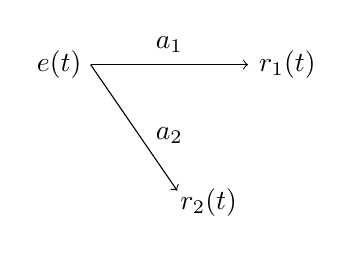
\begin{tikzpicture}
\draw [->] (1,2) -- (3,2);
\draw [->] (1,2) -- (2.1,0.4);

\node[] at (0.6,2) {$e(t)$};
\node[] at (3.5,2) {$r_1(t)$};
\node[] at (2.5,0.25) {$r_2(t)$};
\node[] at (2.0,2.25) {$a_1$};
\node[] at (2.0,1.1) {$a_2$};
\end{tikzpicture}
\end{center}
\end{figure}

Consider an EMI signal $e(t)$ received on two nearby antennas:
\begin{equation}
\begin{split}
r_1(t) &= a_1 e(t) \\
r_2(t) &= a_2 e(t) \\
\end{split}
\end{equation}
where $a_1$ and $a_2$ are complex constants that model path loss and phase shift due to propogation delay. It can be shown that:
\begin{equation} \label{eq_diversity1}
r_1(t) = cr_2(t)
\end{equation}
where $c=a_1/a_2$, the ratio of two complex gains.  Thus if we can estimate $c$, we can use (\ref{eq_diversity1}) to estimate and remove the EMI $r_1(t)$ received on antenna 1. To satisfy (\ref{eq_diversity1}), we need to choose $c$ to minimise the cost function:
\begin{equation} 
E = r_1(t) - cr_2(t)
\end{equation}
This model requires the EMI signal to be present (i.e. above the receiver internal noise) in both received signals. In diversity systems the two antennas are placed some fraction of a wavelength apart. Near field intensity is a strong function of distances of less than one wavelength, so the two antennas are likely to have very different responses to near field EMI. For example at a spacing of $\lambda/4$ a near field signal coupled to one antenna may be undetectable in the other antenna. This implies the effectiveness of diversity will be very sensitive to antenna placement.

When suppressing far field EMI signals amplitude will be less sensitive to antenna placement. However this model also requires that the noise $e(n)$ be a point source.  Consider the case where the there are several independent noise sources $e_n(t)$ located at different locations, e.g. an urban location in the middle of a city.  It is unlikely the phase and amplitude relationships will be the same for each sources so the solution of (\ref{eq_diversity1}) will be different for each source.  If we rely on a single coefficient $c$ cancellation will be ineffective.  So the effectiveness of diversity with rely on how well the noise resolves to a single point source.

\subsection{Directional Antennas}

Consider a isotropic antenna that receives power equally from all directions.  The gain pattern can be visualised as a sphere of constant radius, with a solid angle of $4 \pi$ steradians. Now consider an ideal directional antenna with a cone shaped pattern that receives all it's power from a solid angle of $\theta$ steradians, and no power from any other angle.  It's power gain is $G=\frac{4 \pi}{\theta}$. 

If the EMI is the sum of many sources it is likely to have equal power flux density in all directions.  Consider an isotropic antenna placed at the centre of this field. If the total noise power received from an isotropic antenna is $N$ watts, the noise power in a solid angle of $\theta$ radians is $N \frac{\theta}{4 \pi}$ Watts, and the noise power at the directional antenna terminals is:
\begin{equation}
\begin{split}
 P &= N \frac{\theta}{4 \pi} G \\
   &= N \frac{\theta}{4 \pi} \frac{4 \pi}{\theta} \\
   &= N
\end{split}
\end{equation}
Thus the noise power received by a directional antenna is the same as an isotropic antenna and the same in any direction. In contrast our far field wanted signal is a point source. If that signal develops a power of $S$ watts into an isotropic antenna, it will develop a power of $GS$ watts at the terminals of our directional antenna. The S/N improvement using a directional antenna in a uniform EMI field is therefore improved by the antenna gain $G$.

If the EMI is a point source, we may be able to place it in a pattern null using a directional antenna or diversity/beamforming techniques, further improving the effectiveness of the attack.

\subsection{Topologies}

Antenna topologies may help reduce near field coupling.  For example the conductors of physically small loops and dipoles can be placed further away from near field sources compared to a full length dipole that must extend across the entire width of an urban block \cite{lz1aq}.

There is some experimental evidence that the loop in/on ground topology \cite{k5jy_log}\cite{duffy_lig} increases SNR in suburban locations compared to traditional antennas such as dipoles.  The low gain (e.g. -30 dB) is usable for Rx operation as noise external to the receiver generally dominates system noise figure at HF. So both signal and noise is reduced, and S/N remains the same. It is a balanced design, and the use of common mode chokes on either end of the feedline is recommended.

How this antenna reduces EMI (as implied by the improved SNR) is unclear, but worthy of further investigation. It is possible that compared to a reference dipole, near field noise is reduced as it is attenuated more than desired far field signals by the low (or subterranian) placement of the antenna.  It has some directivity, and a balanced design which is useful in rejecting common mode feedline currents.  It's low placement may also increase physical distance to near field signals such as overhead power lines and nearby houses. 

There are many subjective reports that small loop antennas (either tuned or untuned) provide signficant reductions in EMI, by virtue of lower sensitivity to near electric fields.  However loop antennas are not magic \cite{w8ji_radio_noise}, and perform worse than dipoles in the presence of strong magnetic fields and even at certain distances from electric fields.  Their principle benefit appears to be small overall dimensions, making them easier to position away from near fields radiating from homes and power lines.

It seems likely that antenna topology alone cannot distinguish far field EMI (such as AWGN noise that is the sum of many noise sources in a city) from wanted signals.

\section{Experimental Measurements 1}

In May 2023 I perfomed some measurements at my suburban home.  The goal was to gain experience in measuring EMI and attempt to fit experimental results to the theoretical framework above.

The home is located in Adelaide (population 1.3 million), South Australia and is on a suburban square corner block of 550 \si{\metre\squared}.  Overhead power lines are on two sides, and the suburb is served by VDSL Internet using overhead 70 year old phone lines.  There are two adjacent houses, and the home and it's Southern neighbour have roof mounted solar PV systems.

The station antenna is an inverted V fan dipole with 40m and 20m elements, suspended over the house (and solar panels), the mast and feed point is 9m above ground. It is coupled to 50 ohm coax using a balun at the feedpoint. Subjectively, SSB stations on the 40m band are hard to hear and unpleasant to listen to, and 20m varies between reasonable noise levels and completely unusable (time varying).

\begin{figure}[h]
\caption{Map of the authors home station.  EMI sources are power and xDSL lines, wiring in the home and adjacent homes, and a roof mounted solar PV system.}
\label{fig:home_map}
\begin{center}
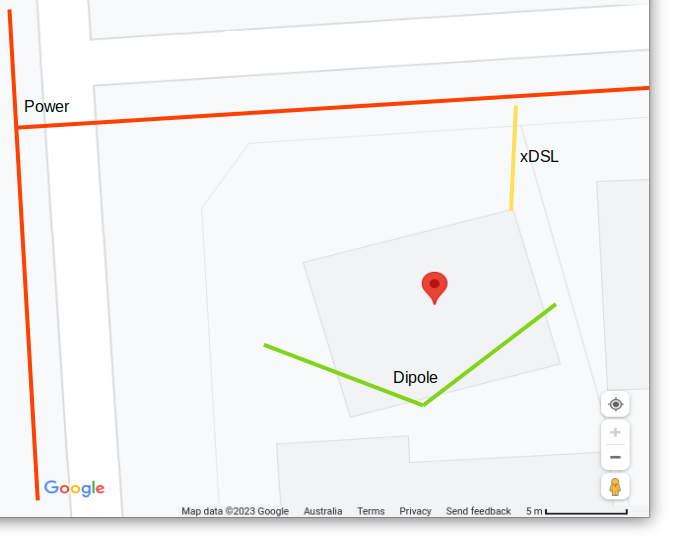
\includegraphics[width=12cm]{house_map.png}
\end{center}
\end{figure}

\subsection{Observations}

\begin{figure}[h]
\caption{Experimental set up for measurements}
\label{fig:meas_config_1}
\begin{center}
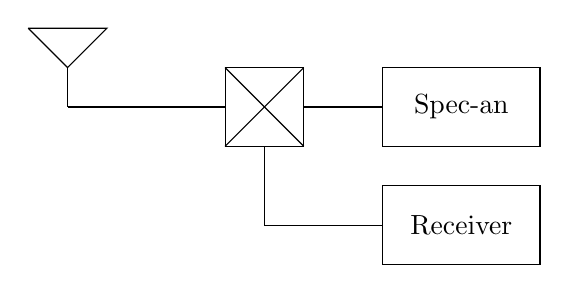
\begin{tikzpicture}
\draw (1.5,3) -- (2.5,3) -- (2,2.5) -- (1.5,3);
\draw (2,2.5) -- (2,2);
\draw (2,2) -- (4,2);
\draw (4,1.5) rectangle (5,2.5);
\draw (4,1.5) -- (5,2.5);
\draw (4,2.5) -- (5,1.5);
\draw (5,2) -- (6,2);
\draw (6,1.5) rectangle (8,2.5);
\draw (4.5,1.5) -- (4.5,0.5);
\draw (4.5,0.5) -- (6,0.5);
\draw (6,0) rectangle (8,1);

\node[align=center] at (7,2) {Spec-an};
\node[align=center] at (7,0.5) {Receiver};
\end{tikzpicture}
\end{center}
\end{figure}

The inverted V dipole was connected via a 3dB splitter to a Rigol DSA 815 spectrum analyser, and the noise power measured at 7.1 and 14.2 MHz.  The spec-an settings were: 3kHz resolution bandwidth, span 200 kHz, pre-amp on, attenuator 0dB, RMS detector, power averaged over 100 counts.  The noise floor of the spec-an is about -160 dBm/Hz. The other port of the splitter was connected to an IC7300 HF radio to monitor the signal.

\begin{figure}[h]
\caption{Scatter plot of noise power measurements over a period of 1 week, made in a 3 kHz resolution bandwidth (top), and converted to a 1 Hz bandwidth at bottom.  Red circles indicate clusters.}
\label{fig:noise_measurements}
\begin{center}
\input measurement.tex
\end{center}
\end{figure}

Figure \ref{fig:noise_measurements} shows noise power measurements were made over a period of one week (1-3 measurements each day) in May 2023 on the 40M and 20M bands.  There were three clusters (Table \ref{table:measurement_clusters}), that were used as a first step in charactering the noise. Each cluster was allocated a label (noise A, B \& C). The external noise figure is given by $F_a = N_0 - 174$. Table \ref{table:external_noise_figure} compares the measurements to the median $F_a$ for residential locations from ITU-R P.372-16 \cite{itu372-16}. The measurements have been adjusted for the splitter (-3.5dB) and feedline (-1dB) losses.  The noise field is assumed to be isotropic so the antenna gain is modelled as 0dB. The measured noise power is consistent my previous efforts using a small tuned loop \cite{rowetel_noise_city}.

Fitting a straight line to the S-unit standard calibration of S9 = -73dBm, and 6dB per S-unit we can find S units from received power $R$ in dBm:
\begin{equation}
S = R/6 + 21.17
\end{equation}
If we assume the receiver sums noise power in a 2000 Hz bandwidth:
\begin{equation} \label{eq:s_unit}
\begin{split}
S &= \frac{N_0+10log_{10}(2000)}{6} + 21.17 \\
S &= N_0/6 + 26.7
\end{split}
\end{equation}
The S units are not sensitive to filter bandwidth, e.g. for a 3000Hz bandwidth $S = N_0/6 + 27$.
\begin{table}[h]
\centering
\begin{tabular}{l c c c c}
 \hline
 Label & Freq (MHz) & $N_0$ (dBm/Hz) & $F_a$ Meas (dB) & S-unit \\
 \hline
 A & 7.1  & -121 & 53 & S6.5 \\
 B & 14.2 & -139 & 35 & S3.6 \\
 C & 14.2 & -125 & 52 & S6.4 \\
\end{tabular}
\caption{Noise sources and equivalent External Noise Figure $F_a$ and S-units.}
\label{table:measurement_clusters}
\end{table}

\begin{table}[h]
\centering
\begin{tabular}{l c c c}
 \hline
 Label & Freq (MHz) & $F_a$ P.372 (dB) & $F_a$ Meas (dB) \\
 \hline
 A & 7.1  & 49 & 53 \\
 B & 14.2 & 41 & 35 \\
 C & 14.2 & 41 & 52 \\
\end{tabular}
\caption{Median P.372-16 Residential External Noise Figure $F_a$ compared to measurements.}
\label{table:external_noise_figure}
\end{table}

\subsection{Discussion}

\begin{enumerate}
\item The IC7300 S-meter was found to be uncalibrated \cite{vu2nsb_s_meter} (6dB power change not equal to one S unit) and could not be relied upon to measure noise power.  Instead, the S-units in Table \ref{table:measurement_clusters} where calulated using equation (\ref{eq:s_unit}). However the IC7300 waterfall is quite useful as a single plot shows both $R<B$ impulse noise (lines across all frequencies) and $R>B$ PWM (harmonics spaced at $R$ Hz).
\item The site has strong 50 Hz impulse noise however the IC7300 noise blanker removes this quite effectively, especially on 7.1 MHz.  The zero span feature of the spec-an (set to 100ms sweep time) is useful for observing these short impulses - it turns the spec-an into a tuned oscilloscope with adjustable centre frequency and bandwidth.  A sweep time of 100ms and resolution bandwidth of 30 kHz was useful for observing 10ms period pulses typical of 50 Hz impulses (one per edge).
\item Noise A/B appeared to be mainly AWGN, although at times PWM harmonics could be observed on both bands. The presence of the harmonics had no affect on the observed noise power between the harmonics, which suggests a small modulation index $h$.
\item The 14.2 high level noise C corresponded to wideband noise with quite wide harmonics about 30kHz apart just visible on the waterfall.  From our PWM analysis in Section \ref{pwm}, this suggests $R>B$ with a fairly high modulation index $h$.  The time varying power between B and C could be due to shifts in the mean PWM duty cycle $d$, leading to shifts in the $sin(\pi n d)$ Fourier coefficients across the observed band.  Given $n$ is so high, even small shifts in $d$ can cause large changes in the amplitudes of the Fourier components.
\item A 500MHz bandwidth oscilloscope with a 50 ohm input was connected instead of the spec-an but was not found to be very useful; nearby AM broadcast stations tend to dominate the wideband time domain signal.  Fitting a 7MHz high pass filter fixed this problem and made the oscilliscope more useful (see below). 
\end{enumerate}

\subsection{Diversity Receiver}

A set of experiments was conducted with the Linrad application \cite{linrad_home} configured to use an Afedri AFE822x Dual channel SDR \cite{afedri_dual}.  The second antenna was a portable end-fed dipole erected in the front of the property, about 10m from the inverted V dipole, sloping from 7m down to 2m.

Due to strong AM broadcast signals beneath 2 MHz, the AFE822x gain had to be reduced to avoid clipping, raising the noise floor of the receiver, and limiting the amount of diversity cancellation possible. The signals from both antennas were often quite different.  This suggests signals local to each antenna such as near field EMI, or feed line pick up.

Using the Linrad phasing feature \cite{linrad_phasing} it was possible to suppress signals that were common to both receivers, for example strong PWM harmonics.  When tuned to segments of the "noise floor", suppression was not possible, which suggests the noise signals being received by both receivers were different.

An experiment was conducted where the signal from one antenna was split, and fed into each receiver.  In this case, the noise could be suppressed by Linrad, demonstrating that if the noise in both receivers satisfies (\ref{eq_diversity1}), it can be cancelled.

\subsection{Conclusions}

\begin{enumerate}
\item Noise A \& B are close to P.372, AWGN in nature, and cannot be reduced further with diversity.  This suggests far field noise from the surrounding city (many sources, many directions), which means I'm doing as well as expected (perhaps a little better than the median at 14.2 MHz).  Turns out I'm normal after all!  Experimentation with antennas is the best way to improve the SNR of received signals. 
\item Noise C on 14.2 MHz look like local PWM noise, and needs further investigation.
\end{enumerate}

\section{Experimental Measurements 2}

Loop Antenna, different positions

\subsection{Observations}

\begin{figure}[h]
\caption{Experimental set up for second set of measurements.  The oscilliscope enables the noise to be observed in the time and frequenmcy domain.  The 7 MHz Band Pass Filter (BPF) removes the strong broadcast signals, making the oscilliscope more useful.}
\label{fig:meas_config_2}
\begin{center}
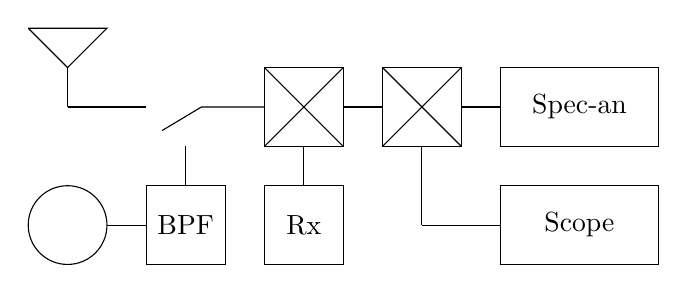
\begin{tikzpicture}

% antenna
\draw (1,3) -- (2.0,3) -- (1.5,2.5) -- (1,3);
\draw (1.5,2.5) -- (1.5,2);
\draw (1.5,2) -- (2.5,2);

% loop antenna
\draw (1.5,0.5) circle (0.5);
\draw (2,0.5) -- (2.5,0.5);

% BPF
\draw (3,1) -- (3,1.5);
\draw (2.5,0) rectangle (3.5,1);
\node[align=center] at (3,0.5) {BPF};

% switch
\draw (2.7,1.7) -- (3.2,2) -- (4,2);

% first splitter
\draw (4,1.5) rectangle (5,2.5);
\draw (4,1.5) -- (5,2.5);
\draw (4,2.5) -- (5,1.5);
\draw (5,2) -- (5.5,2);

% second splitter
\draw (5.5,1.5) rectangle (6.5,2.5);
\draw (5.5,1.5) -- (6.5,2.5);
\draw (5.5,2.5) -- (6.5,1.5);

% Rx
\draw (4.5,1.5) -- (4.5,1);
\draw (4,0) rectangle (5,1);
\node[align=center] at (4.5,0.5) {Rx};

% spec-an
\draw (6.5,2) -- (7,2);
\draw (7,1.5) rectangle (9,2.5);
\node[align=center] at (8,2) {Spec-an};

% scope
\draw (6,1.5) -- (6,0.5);
\draw (6,0.5) -- (7,0.5);
\draw (7,0) rectangle (9,1);
\node[align=center] at (8,0.5) {Scope};

\end{tikzpicture}
\end{center}
\end{figure}


\subsection{Noise D}

An additional noise source D Varies in the range between B and C.  No PWM harmonic structure on the spectogram, but is characterised by powerful time domain impulse when viewed on the oscilliscope.

More obvious on loop, as it's bandwidth is wider.  However buzzy/raspy background noise sound is present on the audio with both antennas.

\subsection{Discussion}

Noise, comes in layers.

\bibliographystyle{plain}
\bibliography{emi_refs}
\end{document}
